
\section{Barrier Certificate Search for First Order 1D System}
A barrier certificate search is tested on the first order system as described in \autoref{subsec:model_1d}, i.e. for the  1D state space system with $x_1\in\mathcal{X}\subset\mathbb{R}$ corresponding to the robot slide joint being the only degree of freedom (see \autoref{fig:safe:overview} for an overview of the slide movement), with a linear position controller as described in \autoref{sec:K_Nbar_1D_1storder}, thus a closed-loop system
\begin{equation}
\dot{x} = \textbf{A}x+\textbf{B}u = \textbf{A}x+\textbf{B}(\bar{\mathbf{N}}x_\text{ref}-\textbf{K}x) = %-\tau^{-1}x+\tau^{-1}u=
-\tau^{-1}x+\tau^{-1}(\bar{\mathbf{N}}x_\text{ref}-\textbf{K}x), \kk \text{with }\tau=110\,\text{ms}\label{eq:sos_firstorder}
\end{equation}
This system is used in the following subsections in the barrier function search.

\subsection{First Order System with Zero Reference}
To give a clear picture of the structure of the \gls{sos} program, an initial exhaustive example is given for the simple 1D first order system with zero as reference position.
Define the open-loop system, and design a controller (with pole placement) as described in \autoref{sec:K_Nbar_1D_1storder}.
\begin{lstlisting}[language=matlab]
% Time constant from measurement
tau = 0.11;
% State-space matrices from first order open-loop system
A = -1/tau;
B = 1/tau;
% Setpoint controller that is xx times faster than the system
xx = 10;
K = place(A,B,[xx*A]);
\end{lstlisting}
Define the desired distance $\Delta$ between the safe and unsafe sets,  the minimum value $\bar{\epsilon}$ of the barrier function on the unsafe set, and the boundaries for each of the three sets $\mathcal{X}$, $\mathcal{X}_u$ and $\mathcal{X}_0$. %in order to get $\mathcal{X} =\{x\in[-0.1,0.1]\}$, $\mathcal{X}_u=\{x\in[0.05,0.1]\}$ and $\mathcal{X}_0=\{x\in[-0.1,0.05-\Delta]\}$.
\begin{lstlisting}[language=matlab]
% scaling factor = 1/100 for [meter], or 1 for [cm]
scale = 1/100;

% Distance between defined safe and unsafe regions
delta = 0.1*scale;

% Minimum value of the barrier certificate on the unsafe set Xu
epsilon = 0.001;

% Set upper and lower limits for the set intervals X, Xu and X0
Xmax = 10*scale;
Xmin = -10*scale;
Xumax = Xmax;
Xumin = 5*scale;
X0max = Xumin-delta;
X0min = Xmin;
\end{lstlisting}

Then the symbolic state variables are declared for the SOS program in SOSTOOLS with the command \texttt{pvar} (which corresponds to the command \texttt{syms} in the MATLAB symbolic toolbox). Now the SOS program \texttt{prog} can be initialized using the function \texttt{sosprogram} which takes the state variable(s) as input. 
\begin{lstlisting}[language=matlab]
% Declare state variables
pvar x1

% Initialize the sum of squares program
prog = sosprogram(x1);
\end{lstlisting}
%The reference for the robot position is generated as the 1D heart position, taking into account the system gain $\bar{N}$, and the closed-loop system equation is written as a function of the sybolic state. %\textcolor{red}{Something is wrong with the reference..?}
The vector field or derivative of the state can now be defined in terms on the symbolic state variable. This function is necessary for the SOS program when requiring that the Lie derivative of the barrier certificate must be negative on the set $\mathcal{X}$.
\begin{lstlisting}[language=matlab]
% Vector field dx/dt = fx (closed loop)
fx = (A-B*K)*x1;
\end{lstlisting}
For ease of defining a (1D) function $g$ that is positive on an interval [$p_1, p_2$], a parabola function is used.
\begin{lstlisting}[language=matlab]
function [a,b,c] = parabola(p1,p2,a)
	if ~exist('a','var')
		a=-1;
	end
	b=a*(p1^2-p2^2)/(p2-p1);
	c=-a*p1^2-b*p1;
end
\end{lstlisting}
Now declare the polynomial barrier function with the command \texttt{sospolyvar}. To do this, a monomial vector must be specified with \texttt{monomials} (see the monomial example in \autoref{eq:monomial_example}), which takes as input the state variable(s) and the monomial degree(s). The monomial degrees for $B(x)$ are chosen as low as possible until a solution can be found. In this case a solution can be found for a degree of $B(x)$ that is 0:4.
\begin{lstlisting}[language=matlab]
% Declare the polynomial barrier function
zB = monomials(x1,0:4);
[prog,Bar] = sospolyvar(prog,zB);
\end{lstlisting}
Now the region $\mathcal{X}$ can be defined for the slide region $\pm0.1$\,m using the Lie derivative inequality in \autoref{cer3_putinar}, which is defined with the command \texttt{sosineq}. The SOS polynomials $q$ are of the form in \autoref{eq:sos_polynomial}, i.e. $q=Z^TQZ$ (so the degree of $q$ is twice the degree of the monomial vector $Z$), and are declared with the command \texttt{sossosvar}, also taking a monomial vector as input.
\begin{lstlisting}[language=matlab]
% Define space X in Rn
[a,b,c] = parabola(Xmin,Xmax); % get coefficients for parabola which is positive for x in [-0.1,0.1] m
gX = a*x1^2+b*x1+c;

zX = monomials(x1,0:4);
[prog,qX] = sossosvar(prog,zX);

prog = sosineq(prog,-diff(Bar,x1)*fx-gX*qX);
\end{lstlisting}
Similarly, the region $\mathcal{X}_u$ is defined according to the SOS inequality in \autoref{cer2_putinar} as the area between slide positions 5-10\,cm.
\begin{lstlisting}[language=matlab]
% Define space Xu in X
[a,b,c]=parabola(Xumin,Xumax);
gXu = a*x1^2+b*x1+c;

zXu = monomials(x1,0:4);
[prog,qXu] = sossosvar(prog,zXu);

prog = sosineq(prog,Bar-epsilon-gXu*qXu);
\end{lstlisting}
And finally the region $\mathcal{X}_0$ is defined according to the SOS inequality in \autoref{cer1_putinar} as $\mathcal{X}_0\subset\mathcal{X}\setminus\mathcal{X}_u$, separated from the unsafe set by the distance $\Delta$.
\begin{lstlisting}[language=matlab]
% Define space X0 in X
[a,b,c]=parabola(X0min,X0max);
gX0 = a*x1^2+b*x1+c;

zX0 = monomials(x1,0:4);
[prog,qX0] = sossosvar(prog,zX0);

prog = sosineq(prog,-Bar-gX0*qX0);
\end{lstlisting}
With all three areas defined according to \autoref{eq:barrier_constraints_putinar}, the program is ready to be solved by using the command \texttt{sossolve}. If a solution is found, an overview of the solution accuracy is printed in the MATLAB terminal as the residual norm, number of iteration steps and solving time. To get the polynomial $B(x)$ use the function \texttt{sosgetsol}.
\begin{lstlisting}[language=matlab]
% Solve for barrier certificate
prog = sossolve(prog);
getB = sosgetsol(prog,Bar)
\end{lstlisting}

\vspace{-2mm}
From the terminal printout it is verified that the problem is neiter primal or dual infeasible, and that the feasibility ratio for this solution is given as 1.0122, which is fairly close to 1 and hence indicates that the solution is valid. The solution is found in 15 iterations with a residual norm of 7.5521e-10 and no indication of numerical errors.

To additionally verify that the solution is indeed valid, it is tested that the solution complies with the inequalities being \gls{sos} by testing if they can be resolved to the form in \autoref{eq:sos_polynomial}.
\begin{lstlisting}[language=matlab]
% Get coefficients for the remaining polynomials
getdBdx = diff(getB,x1)
getqXu1 = sosgetsol(prog,qXu);
getqX01 = sosgetsol(prog,qX0);
getqX1 = sosgetsol(prog,qX);

% Test if the inequalities are SOS
[Q,~,~] = findsos(getB-epsilon-gXu*getqXu1);
[Q2,~,~] = findsos(-getB-gX0*getqX01);
[Q3,~,~] = findsos(-diff(getB,x1)*fx-gX*getqX1);
\end{lstlisting}
%Result
%\begin{lstlisting}[language=matlab]
%Size: 188   33
%
%SeDuMi 1.3 by AdvOL, 2005-2008 and Jos F. Sturm, 1998-2003.
%Alg = 2: xz-corrector, Adaptive Step-Differentiation, theta = 0.250, beta = 0.500
%Put 5 free variables in a quadratic cone
%eqs m = 33, order n = 36, dim = 190, blocks = 8
%nnz(A) = 197 + 0, nnz(ADA) = 493, nnz(L) = 263
%it :     b*y       gap    delta  rate   t/tP*  t/tD*   feas cg cg  prec
%0 :            9.49E-01 0.000
%1 :   9.95E-04 1.03E-02 0.000 0.0109 0.9990 0.9990   1.00  1  1  5.3E-02
%2 :   1.92E-03 2.95E-03 0.000 0.2857 0.9000 0.9000   0.77  1  1  1.9E-02
%3 :   9.73E-03 7.23E-04 0.000 0.2453 0.9000 0.9000  -0.07  1  1  1.4E-02
%4 :   1.64E-01 6.45E-05 0.000 0.0892 0.9900 0.9900  -0.83  1  1  1.7E-02
%5 :   7.57E-01 1.66E-05 0.000 0.2580 0.9000 0.9000  -1.02  1  1  2.0E-02
%6 :   3.17E+00 4.40E-06 0.000 0.2641 0.9000 0.9000  -1.09  3  3  2.0E-02
%7 :   8.00E+00 1.35E-06 0.000 0.3071 0.9038 0.9000  -0.91  1  2  1.8E-02
%8 :   1.16E+01 3.80E-07 0.000 0.2815 0.9132 0.9000  -0.61  2  2  1.1E-02
%9 :   8.37E+00 8.48E-08 0.000 0.2232 0.9000 0.9067   0.05  2  2  3.9E-03
%10 :   4.64E+00 1.41E-08 0.000 0.1661 0.9056 0.9000   0.13  3  3  1.1E-03
%11 :   1.34E+00 2.89E-09 0.000 0.2049 0.9088 0.9000   0.77  4  3  2.6E-04
%12 :   7.91E-02 1.99E-10 0.436 0.0688 0.9900 0.9901   0.91  4  4  1.9E-05
%13 :   7.47E-03 1.24E-11 0.473 0.0624 0.9907 0.9900   0.94  4  4  1.3E-06
%14 :   2.91E-04 5.14E-13 0.486 0.0414 0.9900 0.9900   0.99  4  4  5.5E-08
%15 :   3.18E-06 1.10E-14 0.223 0.0215 0.9900 0.9905   1.01  5  5  1.1E-09
%
%iter seconds digits       c*x               b*y
%15      0.4   7.4  0.0000000000e+00  3.1754678011e-06
%|Ax-b| =   7.6e-10, [Ay-c]_+ =   2.3E-10, |x|=  1.7e+05, |y|=  8.0e+04
%
%Detailed timing (sec)
%Pre          IPM          Post
%6.200E-02    3.130E-01    2.300E-02    
%Max-norms: ||b||=1.000000e-03, ||c|| = 0,
%Cholesky |add|=1, |skip| = 0, ||L.L|| = 9.42104e+12.
%
%Residual norm: 7.5521e-10
%
%iter: 15
%feasratio: 1.0122
%pinf: 0
%dinf: 0
%numerr: 0
%timing: [0.0620 0.3130 0.0230]
%wallsec: 0.3980
%cpusec: 0.4531
%
%
%getB = 
%373.0249*x1^4 + 151.3339*x1^3 + 16.8843*x1^2 - 6.4509e-06*x1 - 0.061301
%
%
%getdBdx = 
%1492.0996*x1^3 + 454.0017*x1^2 + 33.7686*x1 - 6.4509e-06
%\end{lstlisting}

\vspace{-2mm}
This is indeed the case, and it is verified that a barrier certificate is found for the closed-loop system in \autoref{eq:sos_firstorder}, namely
\vspace{-2mm}
\begin{equation}
B(x_1) = 373.0249\cdot x_1^4 + 151.3339\cdot x_1^3 + 16.8843\cdot x_1^2 - 6.4509e\text{-}06\cdot x_1 - 0.061301
\end{equation}

\vspace{-3mm}
The first three coefficients of the polynomial barrier certificate are of ample size (not in the order 1e-5 or less), while the last seem unimportant. Decreasing the degree of the monomial $Z_B$ (and thereby\,the\,order of $B$) to [2:4] does, however, not prove a proper solution, as the inequality \autoref{cer3_putinar} cannot be resolved on the form in \autoref{eq:sos_polynomial} and hence is not \gls{sos}. The  barrier certificate is depicted in \autoref{fig:1D_1stordersys_noRef}.

\begin{figure}[htbp]
\centering%	\hspace*{-12mm}
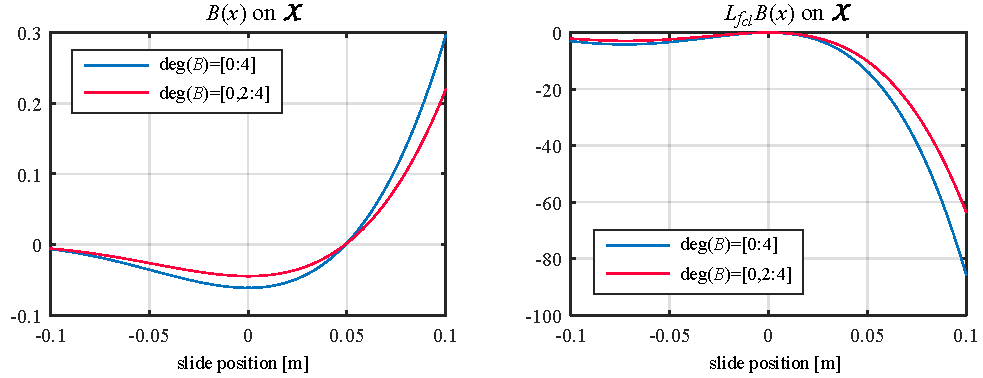
\includegraphics[width=0.9\textwidth]{1D_1stordersys_noRef.pdf}
	\caption{A barrier certificate is found with SOSTOOLS that complies with the requirements in \autoref{eq:barrier_constraints}: it is positive ($B(x_1)\geq \bar{\epsilon}$) on $\mathcal{X}_u=\{x_1\in [0.05,0.1]\}$ and negative on $\mathcal{X}_0=\{x_1\in [-0.1,0.05-\Delta]\}$, and its Lie derivative is nonpositive on $\mathcal{X}=\{x_1\in [-0.1,0.1]\}$.}
	\label{fig:1D_1stordersys_noRef}
\end{figure}












\subsection{Verifying a Range of Reference Positions for the First Order System}

It is desired to verify the system in \autoref{eq:sos_firstorder} for a range of references, preferably for all references within the safe position interval, such that the sets would be as in 

\begin{figure}[htbp]
\centering
\subbottom[]{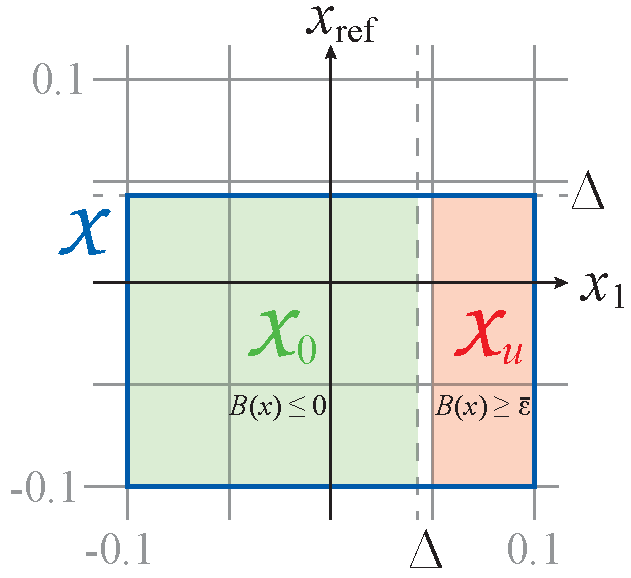
\includegraphics[width=0.3\textwidth]{sos_Xregion.pdf}\label{fig:sos_Xregion}}%
\hspace{3mm}
\subbottom[]{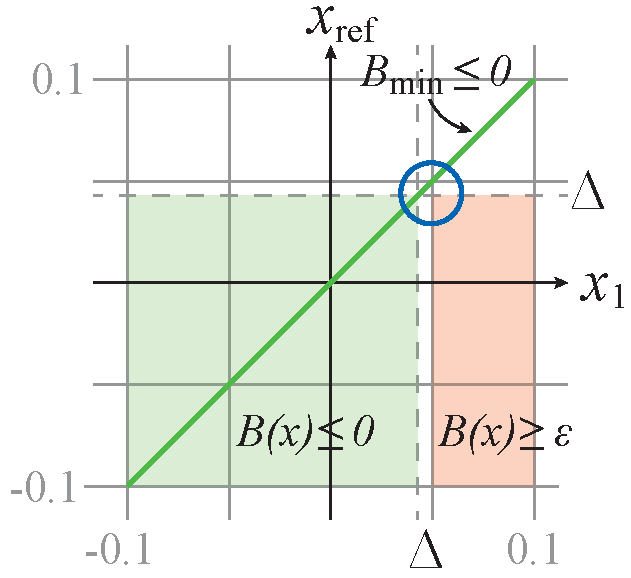
\includegraphics[width=0.3\textwidth]{sos_Xregion_Bvalue.pdf}\label{fig:sos_Xregion_Bvalue}}%
\hspace{3mm}
\subbottom[]{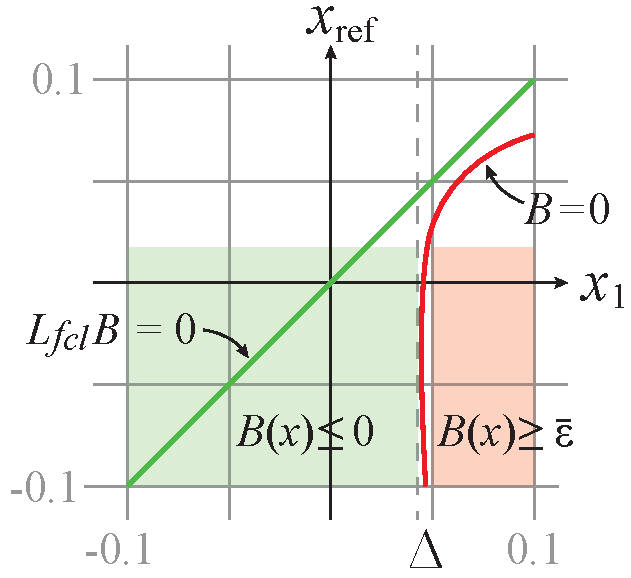
\includegraphics[width=0.3\textwidth]{sos_Xregion_Bvalue_limitref.pdf}\label{fig:sos_Xregion_Bvalue_limitref}}%
\caption{It is desired}
\label{fig:sets_reference}
\end{figure}


Testing with controller k=9 as in the initial design. As the zero reference has proven to point of origin is to test with references in a small interval around zero. $\bar{\epsilon}=0.001$ as before but the safety distance $\Delta$ is increased from 0.001 to 0.002. q degrees 0:4

B degree 0:6 -- ok in interval +-1cm, feas ratio 0.9657, numerr 0, resnorm 6.7e-6. expanding downwards, for -3cm feas ratio 0.8727, to -4cm feasratio 0.9342, for -5 feasratio 0.9321, for -6cm feasratio 0.9579, -10, 1.5cm feasr 0.8377, not workin to 2cm, because the Q not working is that for Xu try to increase $\bar{\epsilon}$ and because numerr is 1 (not workin) also increasing $\Delta$ (also not working). Back to $\bar{\epsilon}=0.001$, $\Delta=0.001$. ok with 1.7cm feasr 0.8259 numerr 0 resnorm 0.00064404, works with 2cm feasr 0.6538 numerr 0 resnorm 0.00087217, not working with 2.5cm (or back down to 2.1cm)


B degree 0:4 -- interval -6, 1cm feas ratio 0.8694, to -7cm feasr 0.9270, -8cm feasr 0.8763 resnorm 0.00027269, -9cm feasr 0.8763, -10cm feasr 0.8255 resnorm 0.00068869, not working with -10, 2cm or with -10,1.5cm, but works with 1.2cm feasr 0.7455 numerr 0 resnorm 0.00060655 "run into numerical problems" (increasing qs to 0:6 still not working with 1.3cm), increasing $\bar{\epsilon}=0.01$ because of numerical problems and resnorm but not working with 1.2cm (also not working when increasing $\Delta=0.01$), but with this delta it works at 0.5cm feasr 0.9030 numerr 1 resnorm 0.0003211, then decreasing delta back not working

try to increase the degree of B and qs drastically, but feasratio becomes negative and Q1 cannot be found (it also takes very long to compute), primal infeasible. Decreasing degrees to B 0:8 and qs 0:6 and $\bar{\epsilon}=0.001$, $\Delta=0.001$ solution found for -10,1.5cm feasr 0.8754, however decreasing degree of qs to 0:4 increases feasr to 0.9458, lowering B to 0:6 feasr 0.8865

or decreasing the region $\mathcal{X}_0$